
\chapter{社会学の成立}

\section{デュルケーム『自殺論』 (1897)}




エミール・デュルケーム (Emile Durkheim, 1858--1917)。


典拠:デュルケーム、『自殺論』、宮島喬訳、中央公論新社、1985。

\subsection{}



〔……〕社会学はみずからによせられている期待にこたえようとすれば、新種の哲学のまがいもの以上になるようにつとめなければならないのである。社会学者は、社会的事実にかんする形而上学的思弁に甘んじないで、はっきりとその輪郭をえがくことができ、いわば指でさししめされ、その境界がどこからどこまでであるかをいうことができるような事実群を、その研究対象とし、断固それにとりくまなければならない。また、歴史学、民族誌、統計学などの補助的な分野をたんねんに参照しなければならない。これらがなくては、社会学は無力なのである。ただなにか懸念される点があるとすれば、それは、これらの科学の明らかにした事実が、にもかかわらず、社会学者の取集しようとしている素材と実際にはなんの関係もないのではないかということである。なぜなら、社会学者がその素材をどれほど注意して限定しようとつとめても、それはきわめて豊富であり、また多様をきわめているので、いわば無限に予想をこえた留保部分をふくんでいるからである。しかし、こんなことは決定的なことではない。もしも、社会学者が、そのような研究方法にしたがうならば、たとえ彼の事実の収集が十分でなく、そのやり方があまりに狭くかぎられたものであっても、ともかく将来にも受けつがれる有益な研究を達成したことになるであろう。というのは、なんらかの客観的基礎をもっている発想は、その創始者の個性に密接にむすびついているということはないからである。それは、なにかしら個をこえたものをもっているので、他の人びともふたたびそれをとりあげて追究することができる。つまり、伝達が可能だということなのだ。こうして、科学的研究においてある一定の連続性が保証されるようになるが、この連続性こそ、科学的作業において、その進歩をうながす条件にほかならない。(11-12)


\subsection{}




私の実践している社会学的方法は一に帰して、社会的事実は物〔ショーズ〕と同じように、いいかえれば、個人の外部にある実在と同じように研究されなければならない、という基本原則の上に立てられている。これほど多くの批判を浴びた原則はないが、またこれほど基本的な原則もない。というのは、要するに、社会学の成立が可能であるためには、社会学が、なによりもまず、ひとつの対象を、それも社会学独自の研究対象をもたねばならないからである。社会学は、他の諸科学の領域には属さないひとつの実在を認識しなければならない。ただし、そのさい、個人の意識のほかには実在的なものがなにもないとすれば、社会学は、それに固有の研究素材を欠くことになるから、存在しなくなる。とすれば、観察の向けられる唯一の対象は、それをおいてほかにないから、個人の心理状態ということになる。ところが、これを扱うのは心理学の仕事なのだ。じっさい、この観点からすれば、たとえば婚姻、家族、宗教などの実質をなすものはすべて、父性愛、孝心、性的欲求、いわゆる社会本能などの個人的欲求のうちにあることになり、それらの制度はこうした個人的欲求に対応したものとみなされる。あのように多様で複雑な歴史的形態をともなって現われているそれらの制度そのものは、なおざりにされ、ほとんど重視されなくなってしまう。それらの制度は、個人の本性の一般的特徴の外面的、偶然的な現われであるから、その一側面にすぎなくなり、なんら特別な研究を必要としないことになる。たしかに、人類のこれらの永遠なる感情が歴史のそれぞれの時点でどのように外部的に現われたかをときおり研究してみるのは、興味つきないことかもしれない。だが、このように外部に現われたものはすべて不完全なものにすぎないから、さして重視することはできないとされる。なるほど、ばあいによっては、それらの外部的形態をとりのぞいたほうが、原型をよく把握できることがある。外部に現われたものの意味はすべて、その原型から派生したものであり、外部に現われたものは、その原型を変形したものなのだから。こうして、この科学〔社会学〕の基礎を個人の心理的構造に求めることはこれをより強固な基礎の上に確立することになる、という口実のもとに、人はこの科学に属する唯一の対象をそれから遠ざけてしまったのである。社会が存在しなければ、社会学も存立できないということ、また存在するものが個人だけならば、社会は存在しないということを人は理解しない。(13-14)

\subsection{}


〔……〕自殺とは、個人の行為にほかならず、個人のみに関係したものであるため、もっぱら個人的要因によって規定されていなければならないかのようにおもわれる。それゆえに、心理学の領域だけに属するようにおもわれる。事実、自殺への決意を説明するさいには、自殺者の気質、性格、生活歴、私生活上の体験などが引合いにだされるのが通例ではなかろうか。

そうした研究方法がどの程度、またどのような条件のもとで妥当するかを、いまここで検討する必要はない。ただ確かなことは、少なくともそれとは全然異なった側面から自殺をとらえることも可能だということである。もしも自殺を、別々に考察されるべき、たがいに孤立した個々の出来事とのみみないで、所与の時間単位内に所与の社会の内部に起こる自殺を全体的に考察してみるならば、こうして得られた全体は、たんなる個々の単位の総和、すなわち寄せ集められた自殺の和ではなく、それ自体が一種独特のsui generis新しい事実を構成していることがみとめられる。それは、統一性と個性をもちそれゆえ固有の性格をそなえている。さらにいえば、その性格はすぐれて社会的なものなのだ。(25)

\subsection{}


〔……〕ここで比較されている三つの期間を通じて、どこの国でも自殺の増加がうかがわれたが、その増加の動きのなかにあっても、それぞれの国民は相互の距離をたもっていた。各国民には、それぞれ固有の増加率があるというわけである。

したがって、自殺率というものは、ひとつの明確に限定された事実群を構成している。それは、この率の不変性と可変性が同時に証明しているとおりである。すなわち、もしも自殺率が、周囲の多様な状況のなかにおいても同時的に存在が認められるような、まぎれもない、相互に関連しあった特性にもとづくものでなかったならば、自殺率の不変性は説明がつかないからである。そしてまた、自殺率の可変性は、それらの特性の固有性と具体性を表現している。なぜなら、それらの特性は、社会そのものの固有の性格に応じて変わるからである。だから、要するに、第3表に示したような統計的データは、それぞれの社会が全体としてこうむっている自殺傾向を表現しているのである。いまここでは、この傾向がなにからなりたっているのかについて、それが固有の実在性をもった集合精神の一種独特の状態であるのか、それとも個人的諸状態の総和を現わしているにすぎないのか、という点にまで言い及ぶ必要はないであろう。後者の仮説は、これまですすめてきた考察とは両立しがたいのであるが、その問題はいまは保留しておき、本論のなかで取り扱いたいともう。これについてどうおもおうとも、とにかく、こうした自殺傾向は、つねになんらかのかたちにおいて実在している。それぞれの社会は、ある一定数の自殺をひき起こす傾向をそなえているのだ。したがって、この傾向こそが社会学に属する固有の研究対象となることができる。(31-32)

\subsection{}



けっきょく、筆者は、次の三つの命題を順次立証してきたことになる。


\begin{itemize}
\item[] 自殺は、宗教社会の統合の強さに反比例して増減する。

\item[] 自殺は、家族社会の統合の強さに反比例して増減する。

\item[] 自殺は、政治社会の統合の強さに反比例して増減する。

\end{itemize}

以上を比較することにより、次のことが明らかになる。すなわち、それらの種々の社会が自殺の抑止作用をもっているのは、それぞれの社会の特殊な性格によるのではなく、それらすべての社会に共通するある原因による、ということである。宗教がその効果をもつのは、宗教感情に特有の性質のためではない。なぜなら、家族社会も政治社会も強く統合されていれば、それと変わらない効果を生むからである。なお、この点は、いろいろな宗教が自殺に作用する仕方を直接に検討したさいにすでに証明したとおりである。他方、家族的関係や政治的関係の与えてくれる自殺への免疫も、それらの関係に特有の要素からは説明されえない。宗教社会も、これらと変わらない特権をもっているからである。その原因は、程度の差はあろうが、これらすべての社会集団が共有している同一の特性にもとめるよりほかない。ところで、その条件を充たす唯一の特性とは、ほかでもない、それらがすべて強固に統合された社会集団をなしているということである。そこで、次のような一般的結論に達する。すなわち、自殺は、個人の属している社会集団の統合の強さに反比例して増減する、と。


ところで、社会の統合が弱まると、それに応じて、個人も社会生活からひき離されざるをえないし、個人に特有の目的がもっぱら共同の目的にたいして優越せざるをえなくなり、要するに、個人の個性が集合体の個性以上のものとならざるをえない。個人の属している集団が弱まれば弱まるほど、個人はそれに依存しなくなり、したがってますます自己自身のみに依拠し、私的関心にもとづく行為準則以外の準則を認めなくなる。そこで、社会的自我にさからい、それを犠牲にして個人的自我が過度に主張されるようなこの状態を、自己本位主義〔エゴイズム〕とよんでよければ、常軌を逸した個人化から生じるこの特殊なタイプの自殺は自己本位的とよぶことができよう。(247-248)

\subsection{}



そこで、前に明らかにした自殺タイプとはきわだった特徴によって区別されるいま一つの自殺タイプが、ここに浮かびあがってくる。前者は過度の個人化から生じるものであったが、それにひきかえ、後者はあまりにも未発達な個人化を原因とする。すなわち、一方は、一部分あるいは全体的に解体にひんした社会が、個人をそこから逸脱するにまかせているために起こる。他方は、社会が個人をあまりにも強くその従属下においているところから起こる。自我がただ自分自身のみの生をいとなみ、自己以外のなにものにも従属しないでいる状態を自己本位主義と名づけたうえは、集団本位主義という言葉が、その反対の状態をあらわすのに適切であるといえよう。すなわち、自我が自由でなく、それ以外のものと合一している状態、その行為の基軸が自我の外部、すなわち所属している集団におかれているような状態がそれである。それゆえ、この強い集団本位主義の結果生じる自殺を、集団本位的自殺とよぶことにする。(265-266)

\subsection{}



ただし、社会が混乱におちいったときは、たとえそれが苦難にみちた危機から生じた混乱であろうと、幸運な、しかし急激な変化をともなう危機から生じた混乱であろうと、しばし社会はこの活動〔個人にたいする規制〕を行使することができなくなる。そして、さきに確認したあの自殺曲線の急上昇は、じつにここから起こってくる。

じっさい、経済的破綻が生じるさいには、ある個人を、それまで占めていた地位からそれ以下の地位ににわかに突き落としてしまうような、一種の没落現象がみられるものである。したがって、そのような個人は、要求を引き下げ、欲求を制し、前よりもいっそう自制することを学ばなければならない。ことかれらにかんしては、社会のはたらきかけの成果も、すべてむだになってしまう。道徳教育は、もう一度はじめからやりなおされなければならない。ところが、社会はただちに個人を新しい生活に順応させることはできないし、また不慣れなさらに激しい緊張を課することに慣れさせることもできない。その結果、個人は、与えられた条件に順応していないし、しかも、そのような予見でさえもかれに耐えがたい思いをいだかせる。この苦悩こそが、個人を駆って、その味気ない生活を{\——}それを実際に味わう以前にさえ{\——}放棄させてしまう当のものなのだ。

しかし、このことは、危機が勢力と富の突然の増大に由来しているときでも、いっこうに変わらない。じっさい、その場合も、生活の諸条件は変わってしまうので、それまで欲求を規制してきた尺度は、もはやそのままではありえなくなる。というのは、その尺度は、各種の生産者に帰せられるべき分配をほぼ規定しているので、社会的な諸手段のあり方が変われば、尺度も変わるからである。こうして段階規定は混乱してしまうが、さりとて、新しいそれが、時をうつさず用意されるわけにもいくまい。人と物が世人の意識によって新たに分類されるまでには、時間を要する。こうして、いったん弛緩してしまった社会的な力が、もう一度均衡をとりもどさないかぎり、それらの欲求の相互的な価値関係は、未決定のままにおかれることになって、けっきょく、一時すべての規制が欠如するという状態が生まれる。人は、もはや、なにが可能であって、なにが可能でないか、なにが正しくて、なにが正しくないか、またなにが正当な要求や希望で、なにが過大な要求や希望であるかをわきまえない。だから、いきおい、人はなににたいしても、見境なく欲望を向けるようになる。この動揺が少しでも深刻になると、それは、各職務への市民の配置を規定している当の原理にまでおよんでいく。なぜなら、社会のそれぞれの部分の関係が、その動揺によって必然的に変化するから、それらのあいだの関係を表現している理念も、もはやそのまま存続するわけにはいかなくなるためである。危機のおかげで特別の利益にあずかった階級は、もはやそれまでのような忍従に甘んじていることはできない。また、そのことへの反動として、その階級のより大きな富をまのあたりにした周囲の者、あるいは下位の階級の者は、ありとあらゆる羨望をそそられる。このように、欲望は、方向を見失った世論によってはもはや規制されないので、とどまるべき限界のどこにあるかを知らない。そのうえ、このときには、一般に活動力が非常に高まっているため、それだけでも、欲望はひとりでに興奮状態におかれている。繁栄が増すので、欲望も高揚するというわけである。欲望にたいして供されるますます豊富な餌は、さらに欲望をそそりたて、要求がましくさせ、あらゆる規則を耐えがたいものとしてしまうのであるが、まさにこのとき、伝統的な諸規則はその権威を喪失する。したがって、この無規制〔デレーグルマン〕あるいはアノミーの状態は、情念〔パッシオン〕にたいしてより強い規律が必要であるにもかかわらず、それが弱まっていることによって、ますます度を強める。(310-311)

\subsection{}



では、この病弊をのぞくことは、どだいむりなのであろか。あるいは一見そう感じられるかもしれない。なぜなら、筆者がこれまで、好ましい影響を与えると証明してきた社会のうち、真の治癒をもたらすようにおもわれるものは、一つもみあたらないからである。しかし、筆者が証明したことは、たとえ宗教、家族、祖国などが自己本位的自殺を抑止することができるとしても、その原因は、それらのおのおのがよび起こす感情の特殊な性質のうちにもとめられるべきではないということであった。むしろ、その原因の効力はすべて、それらが社会をなしているという一般的な事実に由来している。そして、それらが十分に統合された社会、すなわちどの面においても偏りのない社会であるかぎりにおいて、はじめてその効力が発揮される。とすれば、まったく異なった集団でも、それがひとしい凝集力をそなえていさえすれば、同じはたらきをすることができることになる。さて、宗教社会、家族社会、政治社会などのほかにも、これまで問題にされなかったもう一つの社会がある。それは、同種類のすべての労働者、あるいは同じ職能のすべての仲間がむすびついて形成する職業団体ないしは同業組合である。

この社会がそうした役割を果たすのにふさわしいことは、その定義からしても結論される。それは、同じ労働に従事している個人によって構成されているし、かれらの利害は連帯し、一体化してさえいるので、社会的な観念や感情をはぐくむうえでこれほどうってつけの地盤はない。出自、教育、職業などが同一のため、職業活動は共同生活にとってこのうえなく豊富な素材をなしている。そのうえ、同業組合は、過去において自治と組合員にたいする権威を極端なまでに熱望する一個の集合的人格でありえたことをみずから証明しているので、組合員にたいして一個の道徳的環境となることができたことは疑いをいれない。十分に組織された社会においては、私的利益にたいして、社会的利益はつねに尊重されるべき性格と優位性をそなえているが、組合の利益も、労働者の目にこのようなものとして映じなかったはずはない。(484-485)



 \begin{figure}[htbp]
   \centering
   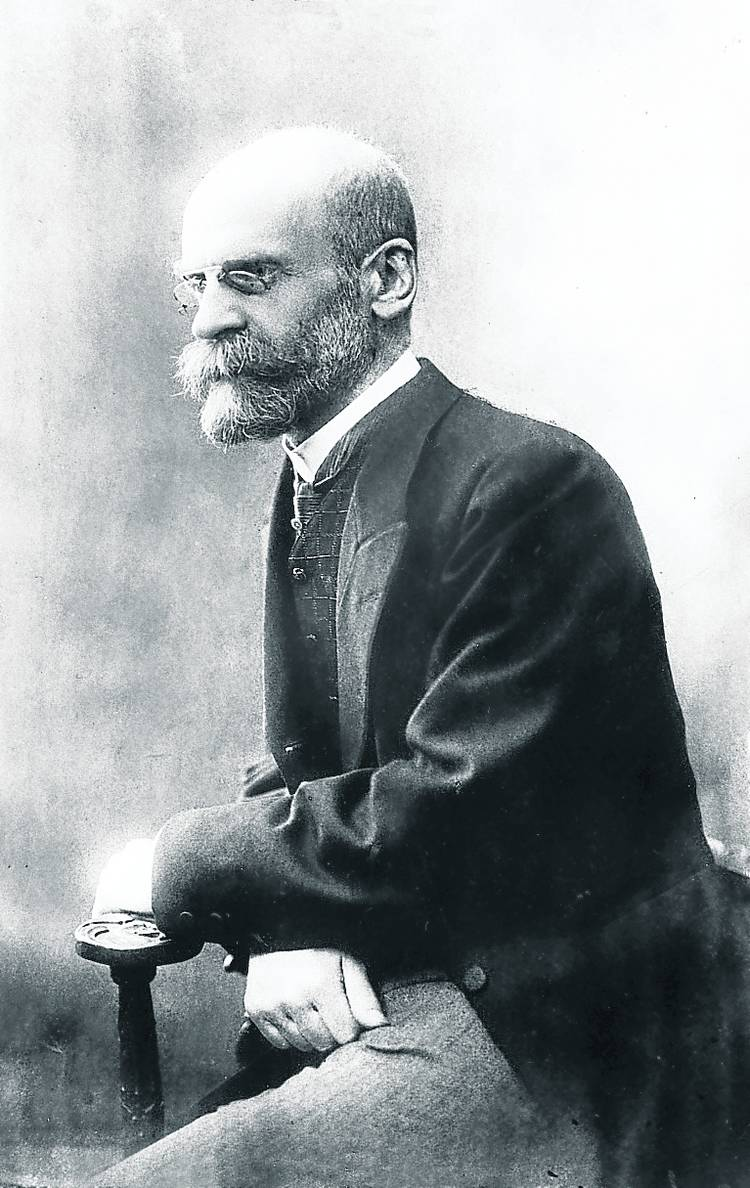
\includegraphics[width=50mm]{images/durkheim.jpg}
   \caption{デュルケーム}
 \end{figure}

\newpage{}

\section{ヴェーバー『社会科学と社会政策にかかわる認識の「客観性」』(1904)}


マックス・ヴェーバー (Max Weber, 1864--1920)。





典拠:マックス・ヴェーバー、『社会科学と社会政策にかかわる認識の「客観性」』、富永祐次・立野保男訳、折原浩補訳、岩波書店、1998

\subsection{}


さて、社会科学的関心の出発点は紛れもなく、われわれを取り囲む社会的文化生活の、\kenten{現実に}、それゆえ個性的に、形成された姿である。社会科学は、この姿の、\kenten{普遍的な}、しかしだからといって\kenten{個性的に}形成されていることにはもとよりいささかも変わりのない連関と、それが、他の、もちろんこれまた個性的性質をそなえた社会的分化状態から生成されてきた経緯とを、究明する。ここには明らかに、われわれがいましがた、天文学を(論理学者にも通例同じ目的で引用される)一極限例として説明した〔個性的実在を、法則を援用して、個性的実在に因果帰属するという〕事情が顕著に看取される。ただし、天文学にとっては、天体が、もっぱらその\kenten{量的な}、精密に計測できる関係において、われわれの関心を引き、考察されるのにたいして、社会科学において問題となるのは、事象の\kenten{質的な}色彩である。その上、社会科学においては、\kenten{精神的}事象の協働が問題となるが、この精神的事象を、追体験しつつ「\kenten{理解する}」ことは、当然ながら、およそ精密自然認識の定式によって解決でき、また解決しようとしているのとは異なる、特殊な性質をそなえた課題である。(77-78)

\subsection{}



さて、以上に述べてきたことの帰結として分かるのは、科学研究の理想的目的は経験的なものを「法則」に還元することでなければならない、という意味で、文化事象を客観的に取り扱うことには意味がない、ということである。そうした取り扱いが無意味であるというのは、しばしば主張されてきたように、文化事象ないしは精神現象が、「客観的」に法則的に生起することがないからではなく、むしろ、(1)社会的諸法則の認識は、社会的実在の認識ではなく、むしろこの〔社会的実在の認識という〕目的のもとに、われわれの思考が用いるさまざまな補助手段のうちのひとつにすぎないからであり、また、(2)いかなる\kenten{文化}事象の認識も、つねに個性的な性質をそなえた生活の現実が、特定の\kenten{個別的}関係においてわれわれにたいしてもつ意義を基礎とする以外には、考えられないからである。ところが、\kenten{いかなる}意味で、また、\kenten{いかなる}関係において、そうである〔生活の現実がわれわれにたいして意義をもつ〕かは、どんな法則によっても、われわれに明らかにされない。というのも、それは、\kenten{価値理念}によって決定されるからであり、われわれは、個々のばあいに、そのつど、この価値理念のもとに「文化」を考察するのである。「文化」とは、世界に起こる、意味のない、無限の出来事のうち、\kenten{人間}の立場から意味と意義とを与えられた有限の一片である。人間が、ある\kenten{具体的な}文化を仇敵と見て対峙し、「自然への回帰」を要求するばあいでも、それは、当の人間にとって、やはり文化であることに変わりはない。けだし、かれがこの立場決定に到達するのも、もっぱら、当の具体的文化を、かれの価値理念に\kenten{関係づけ}、「軽佻浮薄にすぎる」と判断する\kenten{からである}。ここで、すべての歴史的個体が論理必然的に「価値理念」に根ざしている、というばあい、こうした\kenten{純論理的}‐\kenten{形式的}事態が考えられているのである。いかなる\kenten{文化科学}の先験的前提も、われわれが特定の、あるいは、およそなんらかの「文化」を価値があると見ることにでは\kenten{なく}、われわれが、世界にたいして意識的に\kenten{態度}を決め、それに意味を与える能力と意思とをそなえた文化人\kenten{である}、ということにある。(91-93)




  \begin{figure}[htbp]
    \centering
      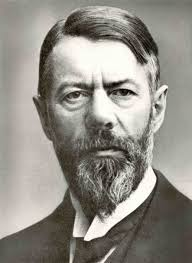
\includegraphics[width=50mm]{images/weber.jpg}
      \caption{ウェーバー} 
  \end{figure}



\section{ウェーバー『職業としての学問』(1916)}



Max Weber (1992). Wissenchaft als Beruf 1917/1919. Politik als Beruf 1919. Wolfgang J. Mommsen \& Wolfgang Schluchter (Hrsg.). Tübingen: J. C. B. Mohr (Paul Siebeck). 

典拠:マックス・ウェーバー、『職業としての学問』、尾高邦雄訳、岩波書店

\subsection{}



職業としての学問の外面的事情については、以上で十分であろう。だが、諸君は実はわたくしからなにかもっとほかのこと、つまり学問を職業とする者の心構えといったようなことについての話を期待しておられたことと思う。ところで、こんにちこの職業にたずさわるものの客観的境遇にとってはともかく、その主観的態度にとって決定的なことは、なによりもまず学問がいまやかつてみられなかったほどの専門化の過程に差しかかっており、かつこの傾向は今後もずっと続くであろうという事実である。こんにちなにか実際に学問上の仕事を完成したという誇りは、ひとり自己の専門に閉じこもることによってのみ得られるのである。これはたんに外的条件としてそうであるばかりではない。心構えのうえからいってもそうなのである。われわれも時折やることだが、およそ隣接領域の縄張りを侵すような仕事には、一種のあきらめが必要である。たとえば、社会学者の仕事は本来こうした性質のものであるが、このばあいかれは、たとえある領域の専門家にたいして、その専門家的見地からは容易に気づかれぬような有益な\kenten{問題提出}をおこなうことがあったとしても、いざこの問題を自分の仕事としてやってみるとき、その結果はきまって不完全きわまるものに終らざるをえないのである。学問に生きるものは、ひとり自己の専門に閉じこもることによってのみ、自分はここに\kenten{のちのちまで残るような}仕事を達成したという、おそらく生涯に二度と味わわれぬであろうような深い喜びを感じることができる。実際に価値ありかつ完璧の域に達しているような業績は、こんにちではみな専門家的になしとげられたものばかりである。それゆえ、いわばみずから遮眼革〔めかくし〕を着けることのできない人々、また自己の全心を打ち込んで、たとえばある写本のある箇所の正しい解釈を得ることに夢中になるといったようなことのできない人は、まず学問には縁遠い人々である。近ごろは学問上の「体験」ということがよく口にされるが、このような人々は、おそらくついに学問を身をもって「体験」することは不可能であろう。こうしたあまり類のない、第三者にはおよそ馬鹿げてみえる三昧境、こうした情熱、つまりいまいったような、ある写本のある個所について「これが何千年も前から解かれないできた永遠の問題である」として、なにごとも忘れてその解釈を得ることに熱中するといった心構え{\——}これのない人は学問には向いて\kenten{いない}。そういう人はなにかほかのことをやったほうがいい。なぜなら、いやしくも人間としての自覚のあるものにとって、\kenten{情熱}なしになしうるすべては、無価値だからである。(21-23)


\subsection{}


学問の進歩は、元来、人類が何千年来それに従ってきた合理化の過程の一部、いな、それのもっとも主要な部分をなすものである。ところが、こんにちでは、一般の人々のこれにたいする態度はいちじるしく否定的である。そこで、われわれはこの学問および学問に裏づけられた技術による主知主義的合理化が、実際にはどのようなことを意味するかを明らかにしよう。

さて、たとえばいまこの講堂におられる諸君は、そのだれもがインディアンやホッテントットのような未開人よりもよく自分の生活条件について知っているといえるであろうか。おそらくは、いなである。たとえばわれわれが電車に乗ったばあい、専門の物理学者なら知らず、一般には、だれもがその動くわけを知らないし、また知らなくてもすむのである。われわれはただそれがどう動くかを「予測」しうればよい。これによってわれわれは、電車の動きにもとづいて行為することができる。しかし、それがどのような構造によって動くかは、少しも知っている必要はないのである。ところが、未開人は、かれらの使用する道具について、これとは比較にならぬほどよく知っている。また、たとえばわれわれが何かを買って金を払うとする。このばあい、いったいどういうわけでこの金というもので{\——}あるときは多くあるときは少なく{\——}物を買うことができるのだろうか。わたくしは受け合っていうが、たとえこの席に経済学の専門家諸君がおられるとしても、これにたいする答えは万人が万人違うであろう。ところが、未開人は、その日その日の食料を得るにはどうすればいいか、またそのばあいにどういう施設が役に立つか、を知っている。それゆえ、主知化し合理化しているということは、それだけたくさん自分の生活条件に関する一般的知識をもっているということでは\kenten{ない}のである。

それは、もっとほかのことを意味する。つまり、それは\kenten{欲しさえすれば}、どんなことでもつねに学び知ることが\kenten{できる}ということ、したがってそこにはなにか神秘的な、予測しえない力がはたらいている道理がないということ、むしろすべての事柄は原則上\kenten{予測}によって\kenten{意のままになる}ということ、{\——}このことを知っている、あるいは信じているというのが、主知化しまた合理化しているということの意味なのである。ところで、このことは魔法からの世界解放(エントツァウベルンク・デア・ウェルト)ということにほかならない。こんにち、われわれはもはやこうした神秘的な力を信じた未開人のように呪術に訴えて精霊を鎮めたり、祈ったりする必要はない。技術と予測がそのかわりをつとめるのである。そして、なによりもまずこのことが合理化の意味にほかならない。

しかし、何千年来西欧文明のうちに受けつがれてきたこの魔法からの解放過程、いいかえれば学問がその肢体ともなり原動力ともなっている「進歩」というものは、はたしてなにか実際上あるいは技術上の意味以上の意味をもつであろうか。諸君は多分この問題が、レオ・トルストイの作品中でもっとも根本的に取り扱われていることを知っておられるであろう。トルストイは、かれ独特のやり方でこの問題に到達している。かれの頭を悩ました全問題は、結局、死とは意味ある現象であるかいなかという問いに帰着する。かれはこれに答えて、文明人にとっては{\——}いなである、という。なぜかといえば、無限の「進歩」の一段階をかたちづくるにすぎない文明人の生活は、その本質上、終りというものをもちえないからである。(31-34)

\subsection{}


もとより、ここに述べたような考えは、人生が、その真相において理解されているかぎり、かの神々のあいだの永遠の争いからなっているという根本の事実にもとづいている。比喩的でなくいえば、われわれの生活の究極の拠りどころとなりうべき立場は、こんにちすべてたがいに調停しがたくまた解決しがたくあい争っているということ、したがってわれわれは、当然これらの立場のいずれかを選定すべく余儀なくされているということ、がそれである。このような事情のもとにあって学問がだれかの「天職」となる価値があるかどうかということ、また学問それ自身がなにかある客観的に価値ある「職分」をもつかどうかということ、{\——}これはまたもやひとつの価値判断であって、この点については教室ではなにごとも発言しえないのである。なぜなら、教えるものの立場にとっては、この点を肯定することがその前提だからである。(65)

\subsection{}


こんにち、究極かつもっとも崇高なさまざまの価値は、ことごとく公の舞台から引きしりぞき、あるいは神秘的生活の隠された世界のなかに、あるいは人々の直接の交わりにおける人間愛のなかに、その姿を没し去っている。これは、われわれの時代、この合理化と主知化、なかんずくかの魔法からの世界解放を特徴とする時代の宿命である。現代の最高の芸術が非公共的であって記念碑的な存在ではないこと、また、かつて嵐のような情熱をもって幾多の大教団を湧きたたせ、またたがいに融合させた予言者の精神に相当するものは、こんにちではもっとも小規模な団体内での人間関係のなかにのみ、しかも最微音(ピアニシモ)をもって脈打っているにすぎないこと、これらはいずれもゆえなきではない。もし記念碑的な芸術品を無理にでもつくろうとしたり、また「発明」しようとしたりするならば、その結果は過去二十年間の多くの記念碑的作品におけるような惨めな出来損ないに終るであろう。また、もしなにか新しい宗教の再興を、しかも新しくかつ真正の予言なしに画策するならば、その結果は、実質的にはやはり同様の出来損ないに終り、しかも前のばあいよりもさらに悪い結果をひきおこすことになるであろう。そして、教壇上の予言は、結局たんなる狂信的諸宗派をつくるだけであって、けっして真の共同体をつくりだしはしないであろう。

\subsection{}



このような時代の宿命に男らしく堪えることのできないものに向かっては、つぎのようにいわれねばならない、かれはむしろだまって、つまり人がよくやるように背教者であることを吹聴して歩くことなく、ただ素直に、またかざり気なく、むかしからの教会の広くまた温かくひろげられた腕のなかへ戻るがいい、と。(71-73)


\vspace{2zw}
\section{推薦図書}




\begin{itemize}
\item 作田啓一(1983)『デュルケーム』講談社。「人類の知的遺産」シリーズの一冊。著者は戦後を代表する社会学者のひとり。(渡)
\item 大塚久雄(1966)『社会科学の方法―ヴェーバーとマルクス―』。(渡)
\item 山之内靖(1997)『マックス・ヴェーバー入門』岩波書店。それぞれの時代を代表する入門書。解釈の変化を知るうえでも併読が望ましい。(渡)
\item 仲正昌樹 (2014) 『マックス・ウェーバーを読む』。ウェーバーの主著数冊のポイントをわかりやすく説明している。この先生の思想史ものはどれもよい。(江)
\end{itemize}



%%% Local Variables:
%%% mode: japanese-latex
%%% TeX-master: "main_gendai"
%%% coding: utf-8
%%% End:
